\documentclass[a4paper]{article}
\usepackage[top=1in,bottom=1in,left=1in,right=1in]{geometry}
\usepackage[utf8]{inputenc}
\usepackage{amsmath}
\usepackage{amssymb}
\usepackage{setspace}
\usepackage{color}
\usepackage{graphicx}
\usepackage{listings}
\usepackage{subcaption}
\usepackage{hyperref}

\setlength{\parskip}{1em}
\setlength{\parindent}{0pt}

\newcommand{\Rbb}{\mathbb{R}}
\newcommand{\Expect}{\mathbb{E}}
\newcommand{\Var}{\text{Var}}
\newcommand{\Cov}{\text{Cov}}
\DeclareMathOperator*{\argmin}{arg\,min}

\DeclareMathOperator*{\argsup}{arg\,sup}
\DeclareMathOperator*{\arginf}{arg\,inf}

% \DeclareMathOperator*{\sup}{sup}

\title{Sensitivity in BNP}
\author{Runjing (Bryan) Liu}
\date{\today}

\begin{document}
\maketitle
\tableofcontents
\newpage

\section{Introduction}
A central question in many probabilistic clustering problems is how many distinct
clusters are present in a particular dataset. In all but the simplest problems,
any attempt to answer this question may be strongly determined by the criterion
used. One common approach, based in the Bayesian tradition, addresses the problem
with a generative model: out of a population of unobserved latent clusters,
some finite number are randomly chosen to be present in the actual data at hand.
The identity and number of these clusters can then be estimated – with attendant
uncertainty estimates – using the tools of Bayesian posterior inference.
For example, one might estimate the “number of distinct clusters present” by its
posterior expectation.
Such a generative model is called a “Bayesian non-parametric” (BNP) model when
the number of latent clusters is infinite, though, naturally, even in
non-parametric models only a finite number of clusters can actually be
observed in any particular dataset.

As with any Bayesian model, this approach requires the specification of a prior
and a likelihood. In this case, the likelihood describes the dispersion of data
within a particular cluster, and the prior determines both the distribution of
cluster shapes and sizes as well as the process that determines how many clusters
are present. In general, different choices of the prior and likelihood would
give different answers to the question “how many distinct clusters are present?”
For example, if the prior does not somehow prefer fewer, larger clusters, then
there is nothing that inherently prevents such an approach from inferring that
each datapoint is in its own cluster. However, one still hopes that a broad range
of reasonable choices of prior and likelihood will come to similar conclusions.
Consequently, it is important, in practice, to measure the sensitivity of the
inferred number of clusters present to the prior and likelihood specification.
Furthermore, these sensitivity measures should work with the kinds of inference
tools that are used in practice, operate relatively automatically without
re-fitting the model many times, and measure sensitivity not only to alternative
hyperparameters but also to alternative functional forms of the prior and likelihood.

To address these needs, we develop fast, automatic measures of the sensitivity of
variational Bayes (VB) approximations to perturbations of functional forms in a putative model.
As a motivating application, we apply our techniques to estimate the sensitivity of BNP posteriors
to the functional form of a particular BNP prior known as the stick-breaking prior.
Stick-breaking priors provide a strong motivation to
quantify functional perturbations. A typical choice of a stick breaking prior is
specified with only a single real-valued hyperparameter and also a potentially
informative distributional assumption, the form of a stick breaking prior can
substantially inform the number of clusters inferred to be present in a particular
dataset, and it is arguably difficult for ordinary practitioners to form meaningful
subjective beliefs about the abstract form of the stick breaking prior.

We begin by deriving a general result for the sensitivity of VB optima to
function-valued perturbations, as well as several useful specializations.
We then describe a VB approximation to a BNP model with a stick-breaking prior and
derive the sensitivity of the approximate number of inferred clusters to the choice of the stick breaking prior.
We then apply our methods to cluster the Iris CITE dataset,
comparing our results to the much more expensive process of re-fitting the model.

\section{Model}
We use the iris dataset CITE, which contains 150 observations of
three different types of iris flowers.
We use measurements of their
sepal length, sepal width, petal length, and petal width to cluster the data with
the goal of recovering the three species. Let $y_{n}\in \mathbb{R}^4$ be these four
measurements for flower $n$.

Let $z_n$ denote the cluster (i.e. the species, which we treat as unknown)
to which flower $n$ belongs.
Each cluster has mean $\mu_k\in \mathbb{R}^4$ and covariance $\Sigma_k \in \mathbb{R}^{4\times 4}$.
Our data generating process is then
\begin{align}
	y_n | z_n \sim \mathcal{N}\Big(\sum_{k=1}^\infty \mathbb{I}\{z_n = k\} \mu_k \;,
              \; \sum_{k=1}^\infty \mathbb{I}\{z_n = k\} \Sigma_k\Big),
	\quad n = 1, ..., N
\end{align}
Note that we allow for an infinite number of clusters. The next section describes
the Bayesian non-parametric prior that makes this possible.

\subsection{The Prior}
We place priors on $\mu_k$, $\Sigma_k$, and $z_n$. \par

We use a Dirichlet stick breaking process CITE as our prior on the cluster components
weights $\pi$, and draw $z_n$ from a multinomial with said weights:
\begin{align}
	\pi &\sim \text{GEM}(\alpha) \label{eq:GEM} \\
	 z_n &\sim \text{Multinomial}(\pi), \quad n = 1..., 150
\end{align}

We can write out equation~\ref{eq:GEM} more explicitly as,
\begin{align}
  \nu_k | \alpha &\sim Beta(1, \alpha) \quad k = 1, .., \infty \label{eq:beta_sticks}\\
  \pi_k | \nu &= \nu_k \prod_{j=1}^{k-1} (1 - \nu_j) \label{eq:stick_breaking}
\end{align}
so posterior inference on the cluster proportions amounts to doing
posterior inference on the sticks $\nu_k$'s.

The other parameters have priors:
\begin{align}
	\mu_k &\sim \mathcal{N}(0, \sigma^2 I_{4\times 4}), \quad k = 1, 2, 3 ... \\
	\Sigma_k &\sim \text{Inv.Wishart}(d, V), \quad k = 1, 2, 3 ...
\end{align}


\section{Variational approximation}
A true BNP representation would take $K = \infty$, but in order to make a computationally feasible
algorithm we truncate $K$ at a value large enough so that many clusters are essentially unoccupied in
the approximate posterior. The variational approximation is
\begin{align}
q(\nu, \mu, \Sigma, z) & =
\Big\{\prod_{k=1}^{K}q\left(\nu_{k}\right)\delta\left(\mu_{k}\right)\delta\left(\Sigma_{k}\right)\Big\} \prod_{n=1}^{150}q\left(z_{n}\right),
\end{align}
where $\delta\left(\cdot\right)$ denotes a point mass at a parameterized
location, $q\left(\nu_{k}\right)$ is a logitnormal distribution, and $q\left(z_{n}\right)$
is a multinomial distribution.

With this variational approximation, we seek
\begin{align}
\eta^* = \argmin_{\eta} KL\Big(q_\eta(\nu, \mu, \Sigma, z) \big\| p(\nu, \mu, \Sigma, z | y)\Big) \label{eq:kl_objective}
\end{align}

where we use $\eta$ to represent the variational parameters be the parameters of the variational distribution
(the mean variance of the logitnormal, the locations of the point masses, etc.).

The posterior quantitiy of interest for us will be the expected number of
clusters under our variational distribution,
\begin{align}
  E_{q(\pi)}\Big[E\Big[\#\{\text{distinct clusters}\}|\pi\Big]\Big] &=
  E_{q(\pi)}\Big[\sum_{i=1}^K P[\text{cluster $k$ is in the dataset}|\pi_k]\Big] \\
    &= E_{q(\pi)} \Big[\sum_{i=1}^K (1 - (1 - \pi_k)^N)\Big]
    \label{eq:expected_num_clusters}
\end{align}

For a given variational distribtion, this quanitity can be computed with
Monte-Carlo draws of sticks $\nu_k$ from the $q(\nu_k)$, and the weights $\pi_k$
are functions of the sticks $\nu_k$ (recall eq. \ref{eq:stick_breaking}).

In the next section we will outline our method for quickly evaluating the
sensitivity of this quantity with respect to various prior perturbations.

% Note that to compute the sensitivity using equation \ref{eq:func_sensitivity},
% we require the derivative
% of this expectation with respect to the variational parameters in $q$. We can compute
% the expectation by sampling the sticks $\nu_k$ from the variational distribution, and
% the cluster weights $\pi_k$'s are functions of the sticks $\nu_k$. Derivatives
% are computed by applying the reparameterization trick to the sticks $\nu_k$.
%

\section{Hyper-parameter Sensitivity}

We consider the effect of perturbing the prior distribution on the sticks.
Let $p_{0k}(\nu_k; \alpha)$ be the $\text{Beta}(1, \alpha)$ prior on the $k$th stick, and
let $p_{\alpha}(\theta | y)$ be the posterior distribution with a particular choice of $\alpha$.
Now the optimal variational parameters also depend on $\alpha$, since $\eta^*(\alpha) =
\argmin_\eta KL(q_\eta\left(\theta\right) \| p_{\alpha}(\theta | y))$.

Now suppose we fit the model at some $\alpha_0$, and we wish to evaluate the
variational parameters should we have chosen a different prior parameter $\alpha_1$.
We can approximate the variational parameters $\eta^*$ at $\alpha_1$ as
\begin{align}
    \eta^*(\alpha_1) \approx \eta^*_{lin}(\alpha_1)
    := \eta^*(\alpha_0) + \frac{d}{d\alpha}\eta^*(\alpha)\Big|_{\alpha=\alpha_0} \cdot (\alpha_1 - \alpha_0)
    \label{eq:our_approximation}
\end{align}

Following CITE,  we compute $\frac{d}{d\alpha}\eta^*(\alpha) $ as:
\begin{align}
  \frac{d}{d\alpha}\eta^*(\alpha)\Big|_{\alpha=\alpha_0} &= H^{-1} f_\eta \label{eq:vb_sensitivty}
\end{align}
where
\begin{align}
  H &= \frac{\partial^2}{\partial^2\eta}\Big\rvert_{\eta = \eta^*, \alpha = \alpha_0}
  KL(q_\eta\left(\theta\right) \| p_\alpha(\theta | y)) \\
  f_\eta &= \frac{\partial^2}{\partial \alpha \partial \eta}\Big\rvert_{\eta = \eta^*, \alpha = \alpha_0} E_{q_{\eta}} \big[\log p_\alpha(\theta)\big]
\end{align}

If $g(\eta)$ is the variational quantity of interest,
e.g. the expected number of posterior quantities in equation \ref{eq:expected_num_clusters},
then we approximate
\begin{align}
    g(\eta^*(\alpha_1)) \approx g(\eta^*_{lin}(\alpha_1))
\end{align}

\subsection{Functional perturbations}
\label{sec:func_pert}
We also consider changing the functional form of the prior on the sticks.
Consider some function $\phi(\nu_k)$, where $\phi(\nu_k) > 0$ for all $\nu_k \in [0, 1]$.
Then we define our contaminated prior on the stick $k$ as

\begin{align}
	\label{eq:expon_perturb}
	p^c_{k}(\nu_k ; \epsilon, \phi) :=
  \frac{p_{0k}(\nu_k)\phi(\nu_k)^\epsilon}{\int p_0(\nu_k')\phi(\nu_k')^\epsilon \lambda(d\nu_k')}
\end{align}
For example, we might consider a different prior for the sticks, say $p_1(\nu_k)$;
letting $\phi(\nu_k) = p_1(\nu_k) / p_{0k}(\nu_k)$,
we are swapping the original prior for a a new prior $p_1$ as $\epsilon \rightarrow 1$.

Here,
\begin{align}
  \frac{\partial}{\partial \epsilon} \log p_k^k(\nu_k | \epsilon, \phi) := \log \phi(\nu_k) -
    \frac{\int p_0(\nu_k')\log\phi(\nu_k')e^{\epsilon\phi(\nu_k')} \lambda(d\nu_k')}{\int p_0(\nu_k')\phi(\nu_k')^\epsilon \lambda(d\nu_k')}
\end{align}
The second term does not depend on $\nu_k$, so $f_\eta = \frac{\partial}{\partial \eta} E_{q_\eta}[\log \phi(\nu_k)]$.

Now if we perturb each stick $k$ by the same perturbation $\phi(\cdot)$, then
and the derivative of $\eta^*$ with respect to this perturbation is given by
\begin{align}
   \frac{d}{d\epsilon}\eta^*(\epsilon) &=
   H^{-1}\frac{\partial}{\partial \eta} E_{q_\eta}\Big[\sum_{k = 1}^K \log \phi(\nu_k)\Big]
  \label{eq:sensitivity_exp_pert}
\end{align}

CITE GUSTAFSON. 

% We have some original $p_0(\theta)$, and suppose we consider a
% ``contaminated prior'' of the form
% \begin{align}
% 	p_c(\theta | \alpha, \phi) :=  \frac{p_0(\theta)(1 + \alpha \phi(\theta))}
% 	{\int p_0(\theta')(1 + \alpha \phi(\theta'))\lambda(d\theta')}
% \end{align}
% We are interested in quantifying the sensitivity to $\alpha$. For example, if we take
% $\phi(\theta) = p_1(\theta) / p_0(\theta)$, then
% \begin{align}
% 	p_c(\theta | \alpha, \phi) :=  \frac{p_0(\theta) + \alpha p_1(\theta)}
% 	{1 + \alpha}
% \end{align}
% and as $\alpha \rightarrow \infty$, we are studying the effect of replacing $p_0(\theta)$ with $p_1(\theta)$.
%
% To evaluate the sensitivity \ref{eq:vb_sensitivty}, we first compute
% \begin{align}
% 	\frac{\partial}{\partial \alpha} \log p_c(\theta | \alpha, \phi) :=
% 		\frac{\phi(\theta)}{1 + \alpha \phi(\theta)}
% 		- \frac{\int p_0(\theta')\phi(\theta') \lambda(d\theta')}{
% 		\int p_0(\theta')(1 + \alpha \phi(\theta'))\lambda(d\theta')
% 		}
% \end{align}
% At $\alpha = 0$, we get
% $\frac{\partial}{\partial \alpha} \log p_c(\theta | \alpha, \phi)
% = \phi(\theta) + 1$.
% Hence, $f_\eta$ is given by
% \begin{align}
% 	f_\eta = \frac{\partial}{\partial \eta} E_{q_\eta}[\phi(\theta)]
% \end{align}
% and following \ref{eq:vb_sensitivty} sensitivity with respect to this contaiminated prior is
% \begin{align}
% 	S^q_\alpha = g_\eta H^{-1}\frac{\partial}{\partial \eta} E_{q_\eta}[\phi(\theta)]
% 	\label{eq:func_sensitivity}
% \end{align}
%
% \subsection{Worst-case perturbations}
% In the previous section, we derived the sensitivity of our prior with respect to a
% particular choice of perturbation $\phi$. In many cases, it is not obvious what
% a choice of $\phi$ should be: hence, we now derive a worst-case choice for $\phi$.
%
% Consider the Hilbert space of $\lambda$-measureable functions, and we
% define the inner product between two functions $a(\theta)$,
% $b(\theta)$ in this space
% as
% \begin{align}
% 	\langle a, b\rangle = \int a(\theta)b(\theta) p_0(\theta) \lambda(d\theta)
% \end{align}
% And we have the corresponding norm $\|a\|_2^2 := \langle a, a\rangle$.
%
% Now we can define the sensitivity from equation \ref{eq:func_sensitivity}
% in terms of this inner product
% \begin{align}
% 	S^q_\alpha &= g_\eta H^{-1}\frac{\partial}{\partial \eta} E_{q_\eta}[\phi(\theta)]\\
% 		&= g_\eta H^{-1}E_{q_\eta}[\phi(\theta) \frac{\partial}{\partial \eta} \log q_\eta(\theta)]\\
% 		&= \langle I(\theta), \phi(\theta)\rangle
% \end{align}
% where
% \begin{align}
% 	 I(\theta) = g_\eta H^{-1}(\frac{q_\eta(\theta)}{p_0(\theta)})\frac{\partial}{\partial \eta} [\log q_\eta(\theta)]
%    \label{eq:influence_fun}
% \end{align}
%
% Now if we define the positive ball of radius $\delta$
% $B_\delta := \{a(\theta) : \|\alpha\| < \delta, \alpha(\theta) \geq \theta, \forall \theta\}$,
% then the worst-case perturbtions are given by
% \begin{align}
%   \label{eq:worst_case_perturbation}
% 	\argsup_{a \in B_\delta} \langle I(\theta), \phi(\theta)\rangle =
% 		\delta\frac{I^+(\theta)}{\|I^+(\theta)\|_2} \quad \text{ and } \quad
% 	\arginf_{a \in B_\delta} \langle I(\theta), \phi(\theta)\rangle =
% 		\delta\frac{I^-(\theta)}{\|I^-(\theta)\|_2}
% \end{align}
% where $I^+(\theta)$ and $I^-(\theta)$ are the positive and negative parts
% of $I(\theta)$, respectively.
%
% \section{Prediction of posterior values}
% Not only do we wish to use the derivative $S^q_\alpha$ to characterize the sensitivity,
% but we also use the derivative and the corresponding linear approximation
% (equation \ref{eq:our_approximation})
% to efficiently approximate posterior quantities should we have
% chosen a different prior, without re-optimizing the variational objective.
%
% Recall that in section \ref{sec:func_pert} we considered a perturbation of the form
% $\phi(\theta) = p_1(\theta) / p_0(\theta)$, and
% \begin{align}
% 	p_c(\theta | \alpha, \phi) :=  \frac{p_0(\theta)(1 + \alpha \phi(\theta))}{\int p_0(\theta')(1 + \alpha \phi(\theta'))\lambda(d\theta')}
% \end{align}
% where $\phi(\theta) = p_1(\theta) / p_0(\theta)$. To replace $p_0(\theta)$ with $p_1(\theta)$, we must take
% $\alpha \rightarrow \infty$,
% and thus a linear approximation, which we only expect to be close for small $\alpha$s,
% will not be sufficient to approximate posterior quantities at $p_1(\theta)$. Hence, we
% consider an alternative parametrization:
% \begin{align}
% 	\label{eq:expon_perturb}
% 	p_c(\theta | \alpha, \phi) :=
%   \frac{p_0(\theta)\phi(\theta)^\alpha}{\int p_0(\theta')\phi(\theta')^\alpha \lambda(d\theta')}
% \end{align}
% so that when $\alpha = 1$, we have that $p_c(\theta | \alpha, \phi) = p_1(\theta)$. We call this
% the {\itshape exponential perturbation}.
%
% Here,
% \begin{align}
%   \frac{\partial}{\partial \alpha} \log p_c(\theta | \alpha, \phi) := \log \phi(\theta) -
%     \frac{\int p_0(\theta')\log\phi(\theta')e^{\alpha\phi(\theta')} \lambda(d\theta')}{\int p_0(\theta')\phi(\theta')^\alpha \lambda(d\theta')}
% \end{align}
% The second term does not depend on $\theta$, so $f_\eta = \frac{\partial}{\partial \eta} E_{q_\eta}[\phi(\theta)]$,
% and the sensitivity is
% \begin{align}
%   S^q_\alpha &= g_\eta H^{-1}\frac{\partial}{\partial \eta} E_{q_\eta}[\log \phi(\theta)]
%   \label{eq:sensitivity_exp_pert}
% \end{align}

% The worst case exponential perturbation is then  given by
% \begin{align}
%   \phi^+(\theta) = \exp\Big\{\frac{I^+(\theta)}{\|I^+(\theta)\|_2}\Big\}
%   \quad \text{ and } \quad
%   \phi^-(\theta) = \exp\Big\{\frac{I^-(\theta)}{\|I^-(\theta)\|_2}\Big\}
%   \label{eq:worst_case_exp_pert}
% \end{align}

% \section{Data}
% We use the iris dataset \cite{iris_dataset}, which contains 150 observations of
% three different types
% of irises: Setosa, Versicolour, and Virginica. We use measurements of their
% sepal length, sepal width, petal length, and petal width to cluster the data with
% the goal of recovering the three species. The data is shown visually in figure \ref{fig:iris_data}.
%
% \begin{figure}[h!]
% 	\centering
% 	\begin{subfigure}[t]{0.4\textwidth}
% 		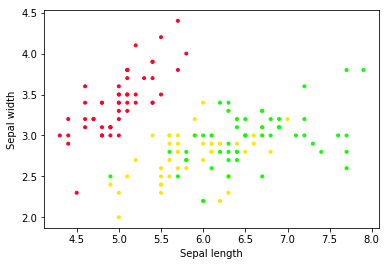
\includegraphics[width = \textwidth]{./data_figs/iris_data.png}
% 		\subcaption{}
% 	\end{subfigure}
%   \begin{subfigure}[t]{0.4\textwidth}
%     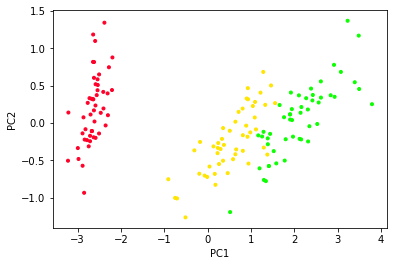
\includegraphics[width = \textwidth]{./data_figs/pca_iris_data.png}
%     \subcaption{}
%   \end{subfigure}
% 	\caption{Visualization of the iris dataset in two dimensions. Points are colored by their
%   true species: red, Setosa; yellow, Versicolour;
%   and green, Virginica. (a) The sepal length against sepal width. (b) The
%   the data projected onto the first two principal components after running PCA.
%   }
% 	\label{fig:iris_data}
% \end{figure}


\section{Results}

\subsection{Parametric Sensitivity}
We first compute a variational approximation to the posterior when the stick breaking
prior parameter is $\alpha = 8.0$. The fit is shown in figure \ref{fig:init_fit}.

\begin{figure}[h!]
	\centering
	\begin{subfigure}[t]{0.4\textwidth}
		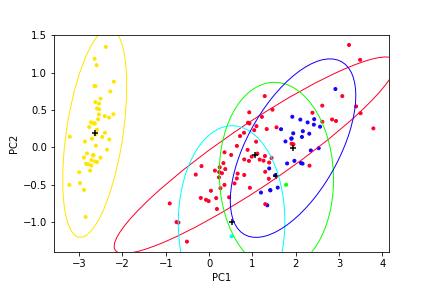
\includegraphics[width = \textwidth]{./parametric_sens_results/init_fit_alpha8.png}
		% \subcaption{}
	\end{subfigure}
	\caption{The data plotted in PC space along the first two principal components, and colored by
	cluster belonging in the model fit. Black crosses are the cluster centroids of the model fit,
  and ovals represent the
  covariances of the model fit. }
	\label{fig:init_fit}
\end{figure}

We seek to evaluate other possible posterior results should we have chosen a different
$\alpha$. The orginal prior for each stick $\nu_k$ has prior
\begin{align}
  p_0(\nu_k) \propto (1 - \nu_k)^{\alpha - 1}
\end{align}
Now if we consider an exponential perturbation (equation \ref{eq:expon_perturb}) and
take $\phi(\nu_k)$ to be $(1 - \nu_k)$,
we have the same effect as perturbing the prior parameter $\alpha$  by $\epsilon$.

% We are particularly interested in investigating the the effect of this prior
% parameter on the expected number of posterior clusters. Our variational
% distribution provides a distribution over the cluster weights $\pi$, induced
% by the distribution on the sticks. We compute the expected number of
% clusters under our variational distribution as
% \begin{align}
%   E_{q(\pi)}\Big[E\Big[\#\{\text{distinct clusters}\}|\pi\Big]\Big] &=
%   E_{q(\pi)}\Big[\sum_{i=1}^K P[\text{cluster $k$ is in the dataset}|\pi_k]\Big] \\
%     &= E_{q(\pi)} \Big[\sum_{i=1}^K (1 - (1 - \pi_k)^N)\Big]
%     \label{eq:expected_num_clusters}
% \end{align}
% Note that to compute the sensitivity using equation \ref{eq:func_sensitivity},
% we require the derivative
% of this expectation with respect to the variational parameters in $q$. We can compute
% the expectation by sampling the sticks $\nu_k$ from the variational distribution, and
% the cluster weights $\pi_k$'s are functions of the sticks $\nu_k$. Derivatives
% are computed by applying the reparameterization trick to the sticks $\nu_k$.

We compare the posterior expectation predicted by our linear approximation against the
expectation obtained from re-optimizing the objective. The results are shown in figure
\ref{fig:parametric_sens_e_num_clusters}.

\begin{figure}[h!]
	\centering
	\begin{subfigure}[t]{0.4\textwidth}
		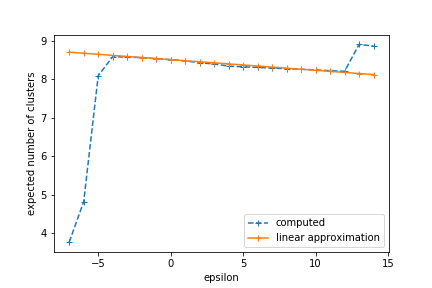
\includegraphics[width = \textwidth]{./parametric_sens_results/pred_num_clusters.png}
		% \subcaption{}
	\end{subfigure}
	\caption{Comparison of the expected number of clusters computed by re-optimizing
  the variational objective for various $\epsilon$ perturbations to the BNP prior parameter
  (blue),
  versus the predicted value from our linear approximation (orange). }
	\label{fig:parametric_sens_e_num_clusters}
\end{figure}

We see that the linear approximation is quite reasonable for $\epsilon \in [-4, 10]$,
but the linear approximation breaks down for larger $\epsilon$.

\subsection{Influence function and worst-case influence}
We compute the influence function of perturbing the DP stick-breaking prior.
Recall that the sticks $\nu_k$ were drawn iid
from a $Beta(1, \alpha)$ distribution.
If we perturb each stick by the same perturbation $\phi(\cdot)$ (in Gustafson style), then the sensitivity is given by
\begin{align}
S_u^q &=
g_\eta H^{-1} \sum_{k = 1}^K \frac{\partial}{\partial \eta} E_{q_\eta(\nu_k)}\Big[\phi(\nu_k) \Big]
\end{align}
where $p_0(\nu_k)$ is the $Beta(1, \alpha)$ pdf. We can now define the {\itshape total} influence function as
\begin{align}
I(\cdot) = g_\eta H^{-1} \sum_{k = 1}^K \frac{q_{\nu_k; \eta}(\cdot)}{p_0(\cdot)}\frac{\partial\log q_{\nu_k; \eta}(\cdot)}{\partial \eta}
\label{eq:total_influence}
\end{align}
where $q_{\nu_k; \eta}$ is the variational approximation specifically for the $k$th stick.

The total influence function is shown in \ref{fig:influence_func}.

\begin{figure}[h!]
	\centering
	\begin{subfigure}[t]{0.4\textwidth}
		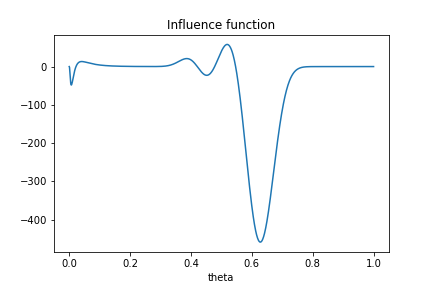
\includegraphics[width = \textwidth]{./func_sens_results/influence_func.png}
		% \subcaption{}
	\end{subfigure}
	\caption{Total influence function of the sticks on the expected number of
  posterior clusters}
	\label{fig:influence_func}
\end{figure}

From the total influence function, we can compute the worst case positive and negative
perturbations (equation \ref{eq:worst_case_perturbation}).
We plot them in \ref{fig:worst_case_perturbations}a-b.

With these worst case functions $\phi^+$ and $\phi^-$, we contaiminate our prior
using the exponential perturbation described in (equation \ref{eq:expon_perturb}).
The contaiminated priors are shown in figures \ref{fig:worst_case_perturbations}.

\begin{figure}[h!]
	\centering
% 	\begin{subfigure}[t]{0.4\textwidth}
% 		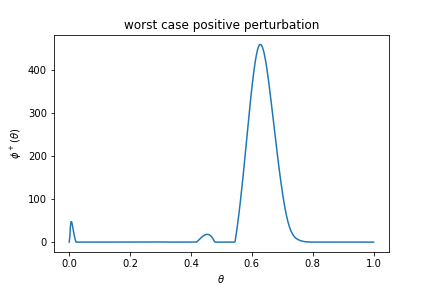
\includegraphics[width = \textwidth]{./func_sens_results/worst_case_neg_pert.png}
% 		\subcaption{}
% 	\end{subfigure}
%   \begin{subfigure}[t]{0.4\textwidth}
%     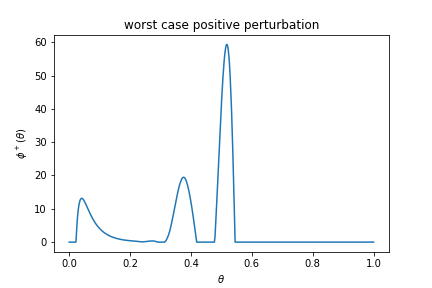
\includegraphics[width = \textwidth]{./func_sens_results/worst_case_pos_pert.png}
%     \subcaption{}
%   \end{subfigure}
% \\
\begin{subfigure}[t]{0.4\textwidth}
  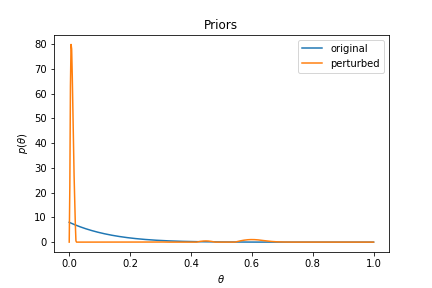
\includegraphics[width = \textwidth]{./func_sens_results/worst_case_neg_priors.png}
  \subcaption{}
\end{subfigure}
\begin{subfigure}[t]{0.4\textwidth}
  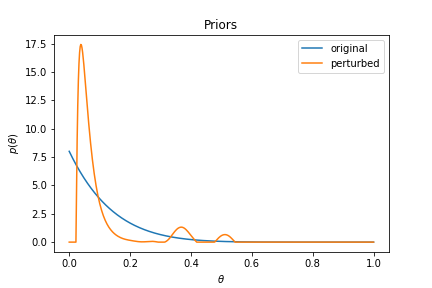
\includegraphics[width = \textwidth]{./func_sens_results/worst_case_pos_priors.png}
  \subcaption{}
\end{subfigure}
	% \caption{(a) and (b), the worst case negative and positive perturbations, respectively.
  % (c) and (d), the original prior in blue; in orange, the prior perturbed (at $\epsilon = 1$) by
  % the worst case negative and positive perturbations, respectively. }
  \caption{The original prior in blue; in orange, the prior perturbed (at $\epsilon = 1$) by
  the worst case negative and positive perturbations, in (a) and (b), respectively. }
	\label{fig:worst_case_perturbations}
\end{figure}

After contaiminating our prior by the worst-case perturbations, we again compute the
expected number of clusters (equation \ref{eq:expected_num_clusters}). We examine the
accuracy of our linear approximation to re-optimizing with the perturbed prior,
in figure \ref{fig:worst_case_results}.

\begin{figure}[h!]
	\centering
	\begin{subfigure}[t]{0.4\textwidth}
		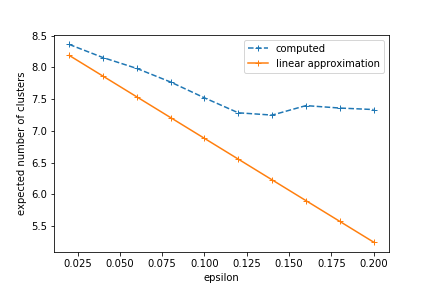
\includegraphics[width = \textwidth]{./func_sens_results/worst_case_neg_influence_results.png}
		\subcaption{}
	\end{subfigure}
  \begin{subfigure}[t]{0.4\textwidth}
    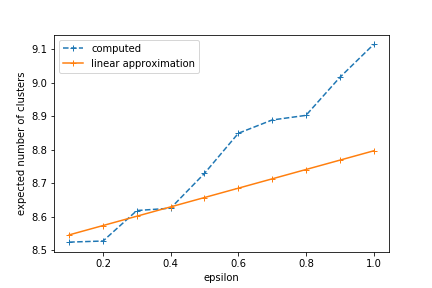
\includegraphics[width = \textwidth]{./func_sens_results/worst_case_pos_influence_results.png}
    \subcaption{}
  \end{subfigure}
  \caption{Expected number of posterior clusters after perturbing by the worst-case
  negative perturbation (a), and the worst-case positive perturbation (b). Blue is the
  expectation obtained from re-optimizing at the contaiminated posterior, while
  orange is the prediction from our linear approximation. }
  \label{fig:worst_case_results}
\end{figure}

\section{Discussion}
In this work, we fit a BNP model to cluster the Iris dataset, and
investigated the sensitivity of the expected number of
posterior clusters to the choice of stick-breaking prior. We proposed an approximate
method that leverages automatic differentiation tools
to efficiently predict the effect of choosing different stick-breaking priors. We show
that for several types of prior perturbations, we were able to provide a reasonable
alternative to the expensive process of re-fitting a variational posterior.


\end{document}
